\section{Methodology (Research Project Details)}
\label{sec:method}

\subsection{Minutiae Detection Network}

We firstly detect the minutiae using deep learning models.
Our basic idea is similar to \cite{AccurateMultiPerson2017}, we first plot a circle with certain radius R (here we set as 10) for each minutiae and then set the pixels ini the circle as 1 and other pixels as 0.
Then we improved it by setting the nearby pixels values as formula \ref{eq:minutiae-circle}.
Here $ r_i $ is the distance between the pixel's position to the \textit{i-th} minutiae location, and $ R $ is a parameter which is used to adjust the circle size in the minutiae heatmap.
It is easy to find that when $ r_i $ equals to $ 0 $, $ v_i $ will be 1, and when $ r_i $ equals to or great than $ R $, $ v_i $ will be 0.
Therefore, only the pixels within the distance of $ R $ of a minutiae has a positive value, and the value of the other pixels will be 0.
If one pixel are in the nearby circles of two or more minutiae, the value will still be 1.


\begin{equation}
    \label{eq:minutiae-circle}
    v = \min(v_i, 1) = \min(\sum_{i}\frac{1}{1 + e^{-0.5*(r_i-R)} - e^{R/2}}, 1)
\end{equation}

Here we performed experiments using many kinds of deep learning structures: such as AutoEncoder, fully convolutional network (FCN) \cite{FCN}, DeepLab v3 \cite{DeepLab-v3} and UNet \cite{unet}, and finally find that UNet can achieve the highest accuracy.
Therefore we finally use UNet to locate the minutiae, and Fig. \ref{fig:unet} presents the basic structure of our minutiae detection network.
Similar to AutoEncoder, this network can be divided into two parts: encoder and decoder.
The encoder downsample the augmented fingerprint images (with a size of $ 560*400 $ ) to extract the feature while the decoder upsample those feature to generate a same size segmentation map.
There are some shortcut connections between the encoder and the decoder, which can bypass more information to the decoder layer.

\begin{figure}[htbp]
    \centering
    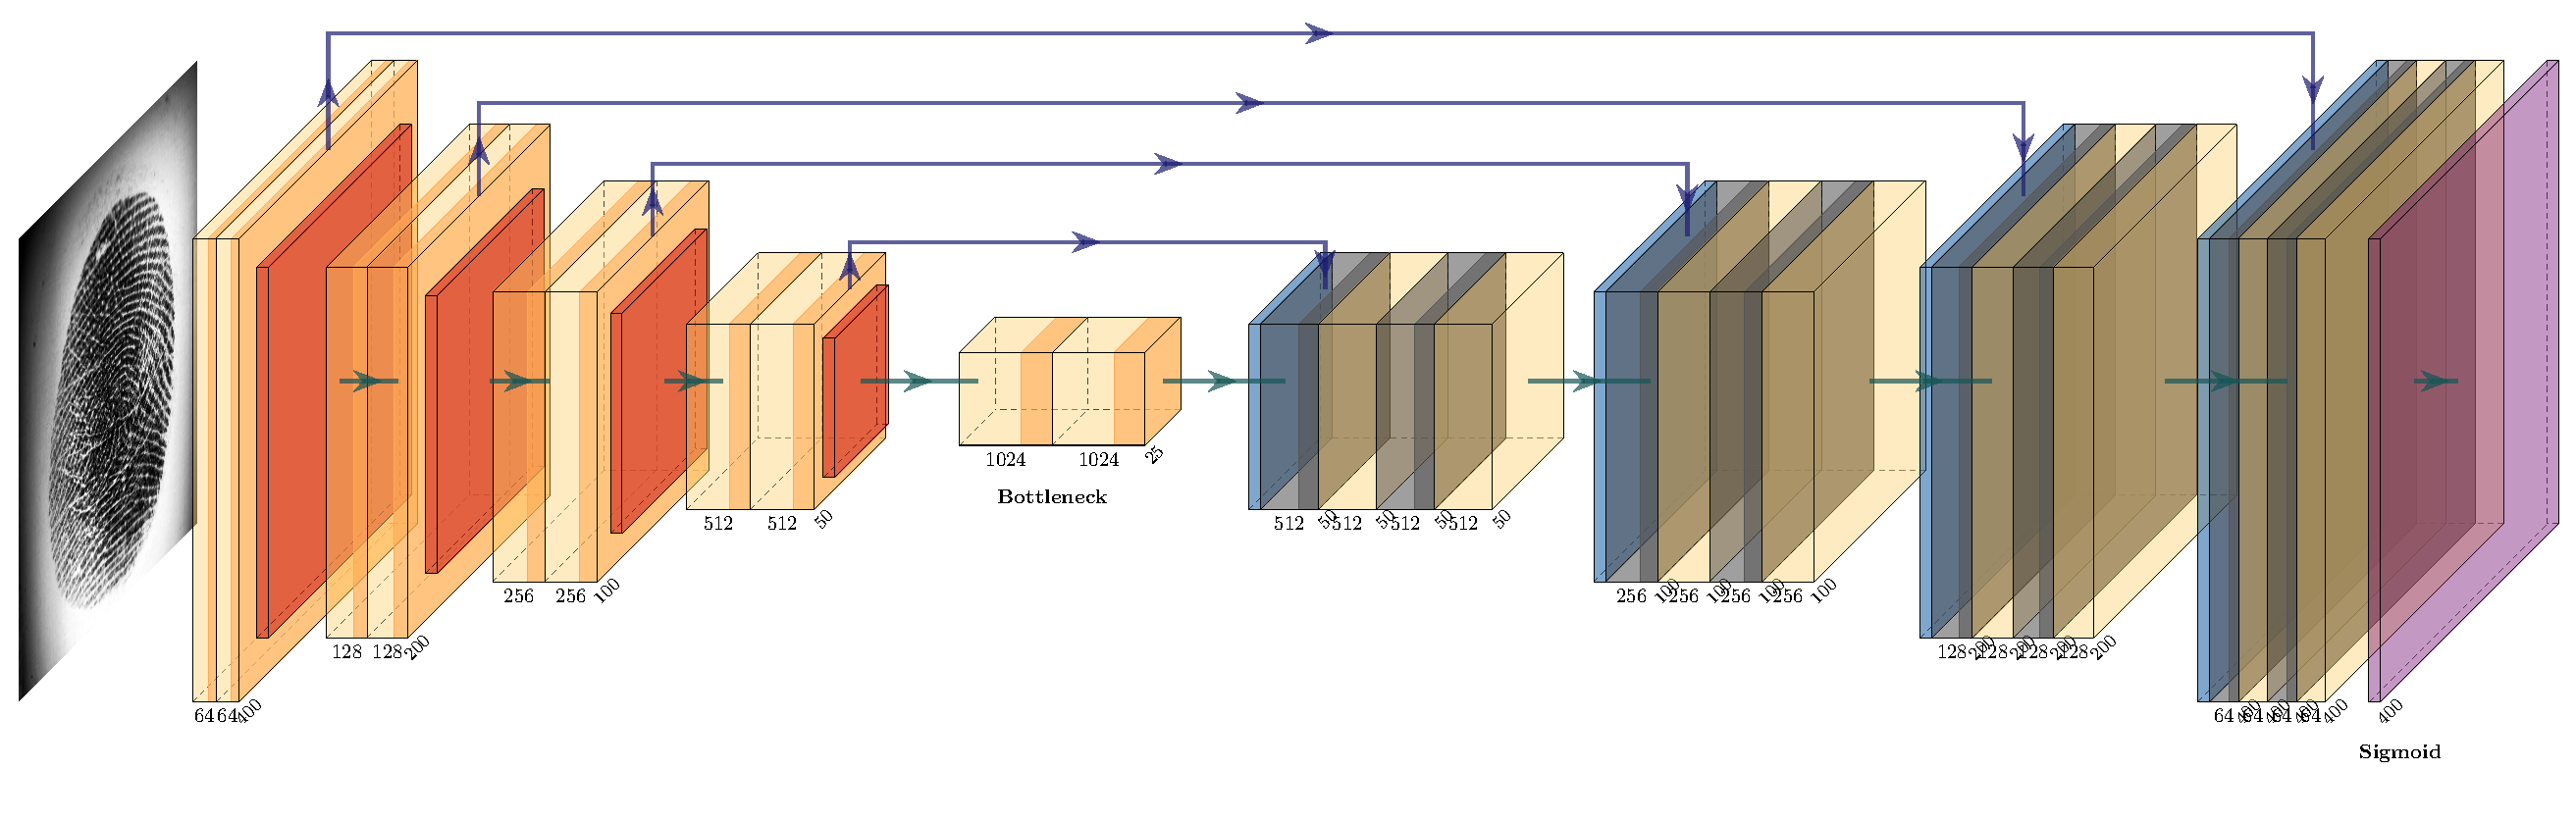
\includegraphics[width=.9\linewidth]{fig/unet.pdf}
    \caption{The structure of our minutiae detection network, plotted with \cite{PlotNeuralNet}}
    \label{fig:unet}
\end{figure}

We does not use normal UNet structure, but use the ResNet18 as encoder or backbone, which is similar to \cite{linknet}.
In addition, we use pre-trained weights in imagenet for the backbone initialization rather than train from scratch, because we find it takes much more time to converge when training from scratch.
It should be noted that we output only one layer and use the sigmoid as the final layer's activation function, which is mainly because that the output minutiae map is binary and it is not useful to use softmax function.
Therefore, we use sigmoid function to limit the output probability into the interval of $ [0, 1] $, and then use binary cross entropy loss as the criterion loss function.

After calculate the minutiae map, we then need to locate the minutiae and output corresponding coordinates.
%  we use the non maximum suppression to locate the minutiae.


\subsection{Minutiae Feature Network}

\begin{figure}[htbp]
    \centering
    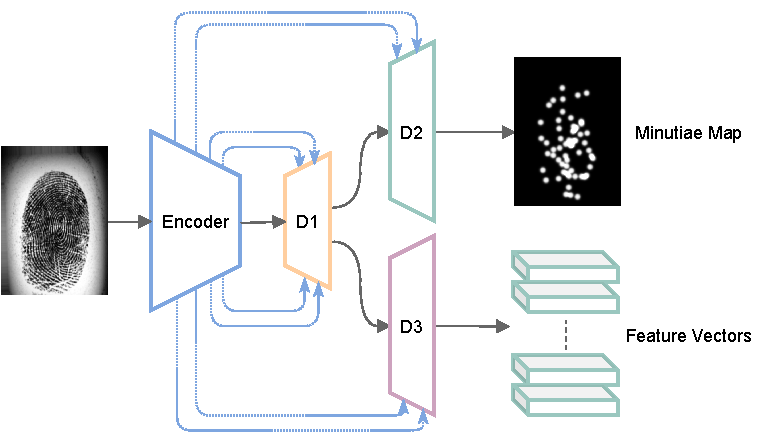
\includegraphics[width=.9\linewidth]{fig/network-structure.pdf}
    \caption{The structure of the minutiae feature network, Encoder and D1 is both used }
    \label{fig:feat-net}
\end{figure}

After detecting the minutiae, we then need to calculate a feature vector for every minutiae.
And we use unet to calculate the minutiae too.
To save both the training time and computation time, we use a part of the minutiae detection network.
Fig \ref{fig:feat-net} presents the structure of our model.
Encoder an D1 are shared between minutiae detection network and minutiae feature network.
D2 are used to train the minutiae map while D3 are used to calculate the feature vector of every minutiae.
Similar to minutiae detection network, the minutiae feature network also output a feature map (size is width*length*feature-channels) where every pixel has its own feature.
Then we select a $ 32*32 $ square patch centered on the minutiae point and calculate the average feature vector as the minutiae feature.

We trained the minutiae detection network first until it converges.
Then we fixed the network weights of the Encoder and D1 and train D3 separately.
Here we incorporated triplet loss function with the cosine distance during the network training.
The triplet loss \cite{SchroffCVPR2015facenet} was originally proposed in the face recognition area but it has shown to work well in other computer vision domain too.

This loss function can be defined as follows.

\def \newf {\mathcal{F}}

\begin{equation}
	\sum_{i=0}^{n}[\newf(x_i^a, x_i^p) - \newf(x_i^a, x_i^n) + margin]_+
	\label{for:triplet-loss}
\end{equation}

where $x_i^a$, $x_i^p$ and $x_i^n$ respectively represent the feature vector of anchor, positive and negative sub-images.
While $\newf$ is the cosine distance function between the two feature vectors as defined in the following.

\begin{equation}
	\newf(x^u, x^v) = \frac{\sum_{i=0}^{n}(x_i^u \times x_i^v)}{\sqrt{\sum_{i=0}^{n}((x^u_i)^2)} \times \sqrt{\sum_{i=0}^{n}((x_i^u)^2)}}
	\label{for:cos-triplet-loss}
\end{equation}

To construct triplet pairs for training, we first randomly select a minutiae from the dataset as anchor data, then we find its corresponding minutiae in another images of the same subject using Minutia Cylinder Code (MCC) \cite{CappelliTPAMI2010mcc} and use it as the positive minutiae, finally we randomly select a minutiae from fingerprint images of other subjects as the negative.


\subsection{Minutiae Graph}
To build minutiae graph, we need to determine vertex and edge for the graph. The most intuitive way to determine the vertex is by choosing the minutiae as the vertex. Here, each vertex is represented by the minutiae pixel location $(x, y)$ from the original fingerprint image. For the edge configuration, there are two ways to connect the vertices by edges. One way is to connect each vertex with its $k$ nearest neighbor and the number $k$ is preset by the user. However, this method is sensitive to missing or spurious minutiae. The other way is to connect the vertices through triangulation. We use Delaunay triangulation method to form the edges here.

\begin{figure*}[!ht]
    \centering
    \begin{minipage}[b]{0.93\linewidth}
        \subfloat[original fingerprint iamge and detected minutiae]{
            \begin{minipage}[b]{0.27\linewidth}
                \centering
                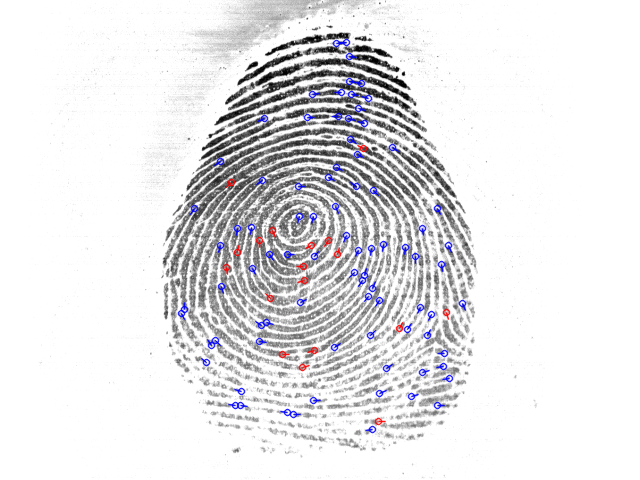
\includegraphics[height=4.0cm]{./image/fingerprint1_1/mnt_overlay.png}\vspace{8pt}
                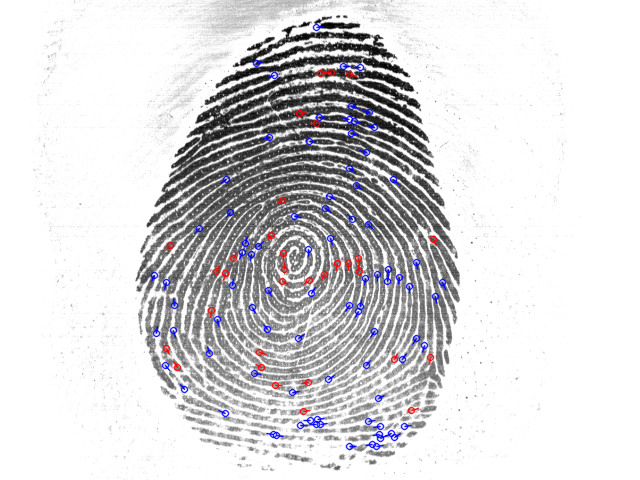
\includegraphics[height=4.0cm]{./image/fingerprint1_2/mnt_overlay.png}\vspace{8pt}
                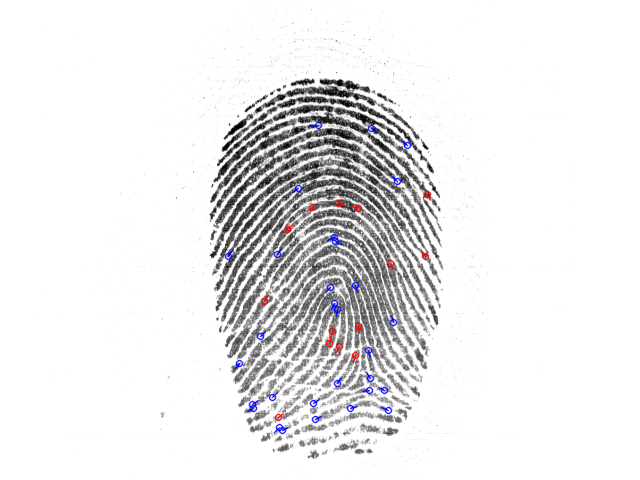
\includegraphics[height=4.0cm]{./image/fingerprint2_1/mnt_overlay.png}
            \end{minipage}
        }
        \hfill
        \subfloat[minutiae connected by triangulation]{
            \begin{minipage}[b]{0.27\linewidth}
                \centering
                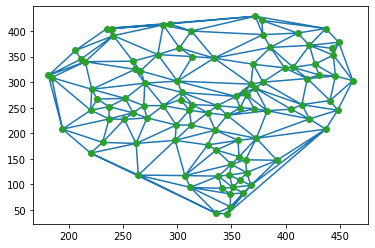
\includegraphics[width=\linewidth, height=4.0cm]{./image/fingerprint1_1/triangulation.png}\vspace{8pt}
                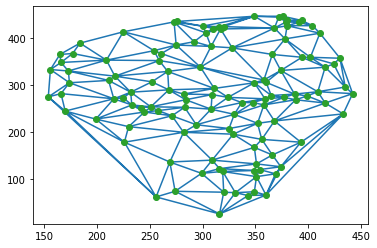
\includegraphics[width=\linewidth, height=4.0cm]{./image/fingerprint1_2/triangulation.png}\vspace{8pt}
                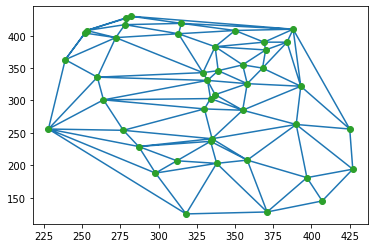
\includegraphics[width=\linewidth, height=4.0cm]{./image/fingerprint2_1/triangulation.png}
            \end{minipage}
        }
        \hfill
        \subfloat[minutiae graph visualization]{
            \begin{minipage}[b]{0.27\linewidth}
                \centering
                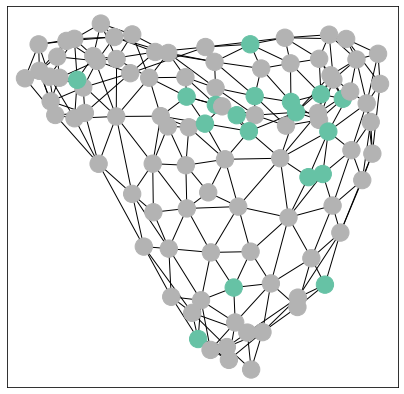
\includegraphics[width=\linewidth, height=4.0cm]{./image/fingerprint1_1/mnt_graph.png}\vspace{8pt}
                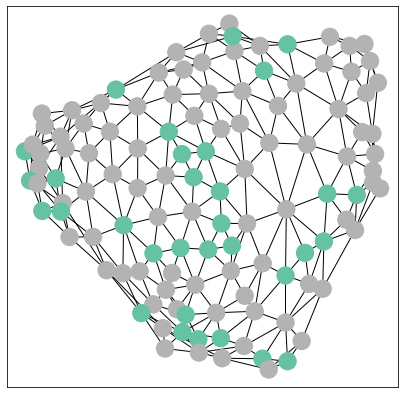
\includegraphics[width=\linewidth, height=4.0cm]{./image/fingerprint1_2/mnt_graph.png}\vspace{8pt}
                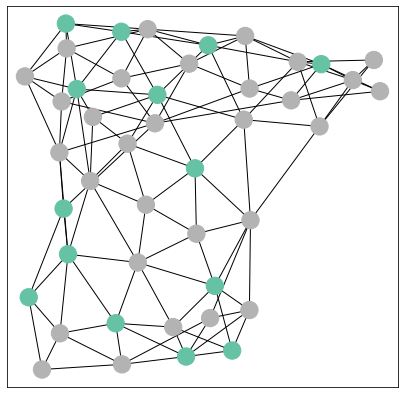
\includegraphics[width=\linewidth, height=4.0cm]{./image/fingerprint2_1/mnt_graph.png}
            \end{minipage}
        }
    \end{minipage}
    \vfill
    \caption{Sample fingerprint and its corresponding minutiae graph}
    \label{fig:mnt}
\end{figure*}

Figure \ref{fig:mnt} illustrates the way we build the minutiae graph. Each row shows one sample fingerprint image with detected minutiae and its corresponding minutiae graph. The left column shows the original fingerprint with detected minutiae that are plotted on it. The middle column shows the minutiae that are connected by Delaunay triangulation method. Note that because the origin of the fingerprint image is on the top left and the origin of the plot is on the bottom left, the minutiae that are plotted in the middle column are turned upside down compared with those minutiae in the left column. The right column shows the minutiae graph once the vertices and edges are built from the previous two columns. The geometric information of the minutiae is lost in the minutiae graph.


\subsection{Data Augmentation}

\begin{figure}[htbp]
    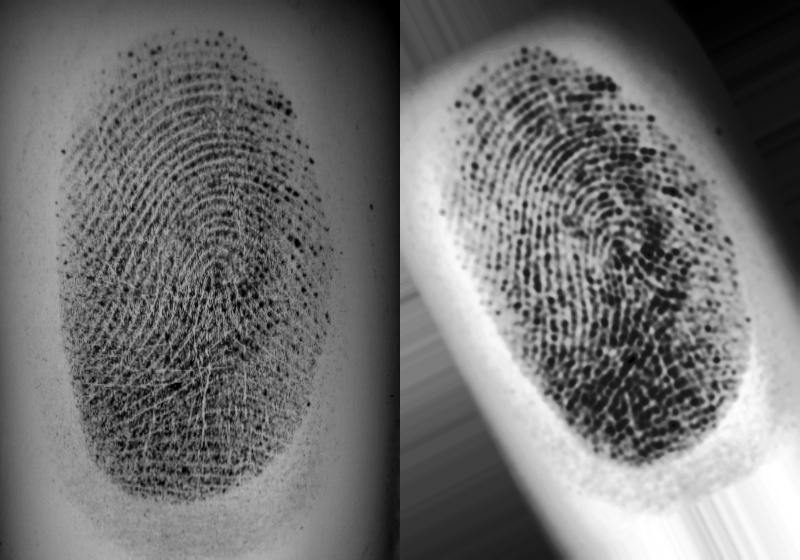
\includegraphics[width=.32\linewidth]{fig/augmentation/aug-1.jpg}
    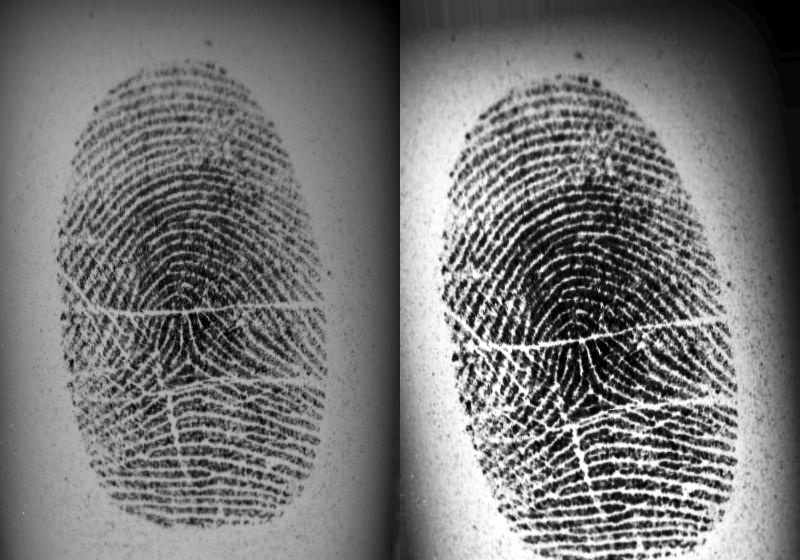
\includegraphics[width=.32\linewidth]{fig/augmentation/aug-2.jpg}
    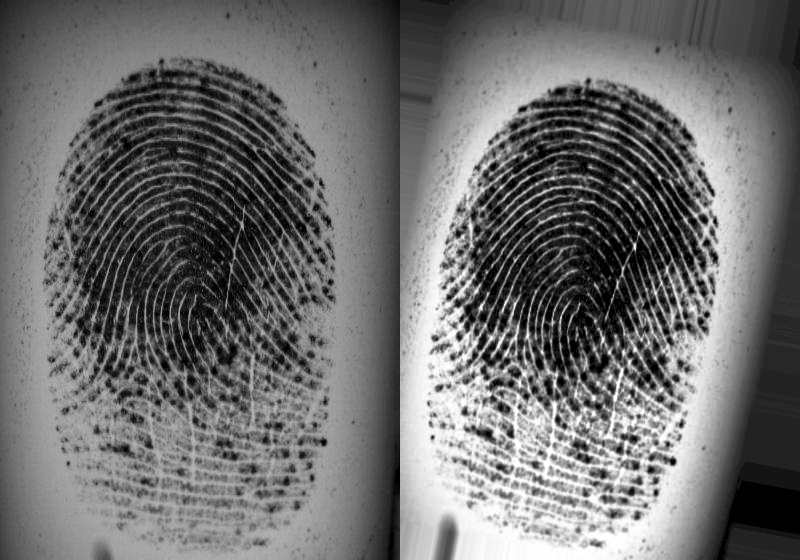
\includegraphics[width=.32\linewidth]{fig/augmentation/aug-3.jpg}
    \newline
    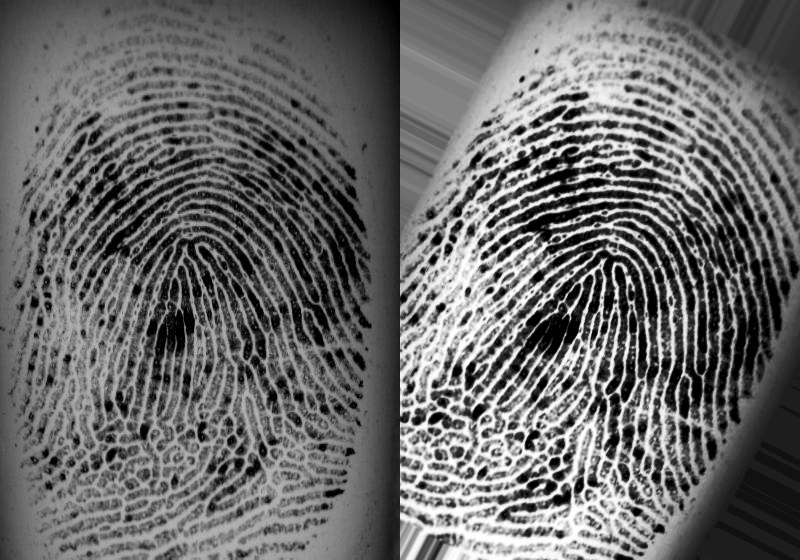
\includegraphics[width=.32\linewidth]{fig/augmentation/aug-4.jpg}
    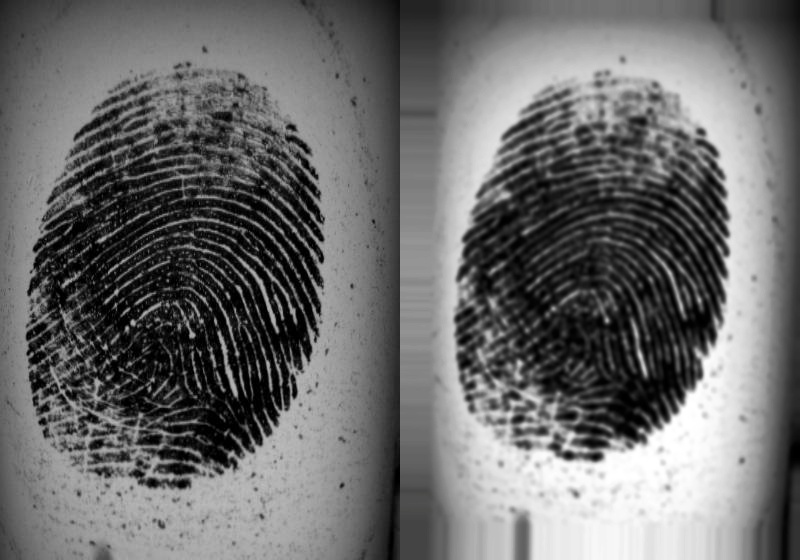
\includegraphics[width=.32\linewidth]{fig/augmentation/aug-5.jpg}
    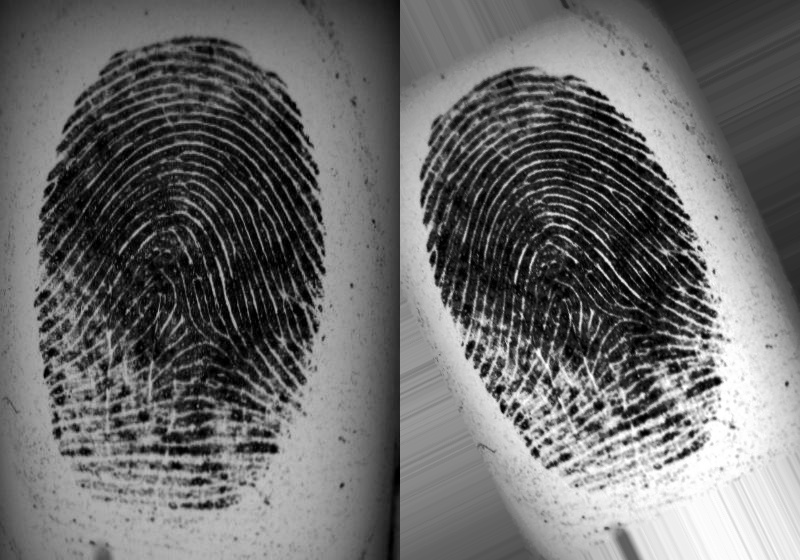
\includegraphics[width=.32\linewidth]{fig/augmentation/aug-6.jpg}
    \caption{Augmentation images samples, left are the original images while right are the augmented images}
    \label{fig:augmentation}
\end{figure}

It is worth to mention that we also do some data augmentation in our experiment to improve the robustness and accuracy.
We use imgaug \cite{imgaug} library in this experiment.
And mainly use the following transforms: random brightness, gamma contrast, Gaussian blur and shift scale rotate.
After the data augmentation, we add a histogram equalization to normalize the images.
Fig \ref{fig:augmentation} presents some sample data augmentation images pairs, where the left is the original fingerprint image and the right is the augmented image.



